\lstset{
	language=[Visual]C++,
	keywordstyle=\bfseries\sffamily\color[rgb]{0,0,1},
	identifierstyle=\sffamily,
	commentstyle=\color[rgb]{0.133,0.545,0.133},
	stringstyle=\sffamily\color[rgb]{0.627,0.126,0.941},
	showstringspaces=false,
	basicstyle=\small,
	numberstyle=\footnotesize,
	numbers=left,
	stepnumber=1,
	numbersep=10pt,
	tabsize=2,
	breaklines=true,
	prebreak = \raisebox{0ex}[0ex][0ex]{\ensuremath{\hookleftarrow}},
	breakatwhitespace=false,
	aboveskip={1.5\baselineskip},
	columns=fixed,
	upquote=true,
	extendedchars=true,
}

\pagebreak
\section{Auto Triggering Function Generator\label{cp:AutoTriggeringFunctionGenerator}}
Some applications require internal periodic or random triggering. The \deviceName\ function generator provides this functionality.\par

The delay between two trigger pulses of this trigger generator is the sum of two components: A fixed value M and a pseudo random value given by the exponent N. \par

The period is

\begin{align}
    T = 1 + M + [1...2^N]
\end{align}

clock cycles with a duration of $4 ns$ per cycle.\par

The trigger can be used as a source for the TiGer unit (see Section \ref{cp:tiger}).


\section{Timing Generator (TiGer)\label{cp:tiger}}
Each LEMO-00 input can be used as a LVCMOS trigger output. The TiGer function can be configured independently for each LEMO-00 connector. 
Each TiGet block can use an arbitrary combination of inputs to trigger its state machine including the AutoTrigger.
See Section \ref{cp:tigerblock} for a full description of the configuration options.

%
\begin{figure*}[ht]
    \begin{center}
        \ifxHPTDC {
            % this is an XCIrcuit drawing  convertex from postscript with 
            %ps2pdf.exe -dEPSCrop xhptdc8_trigger_matrix.ps
            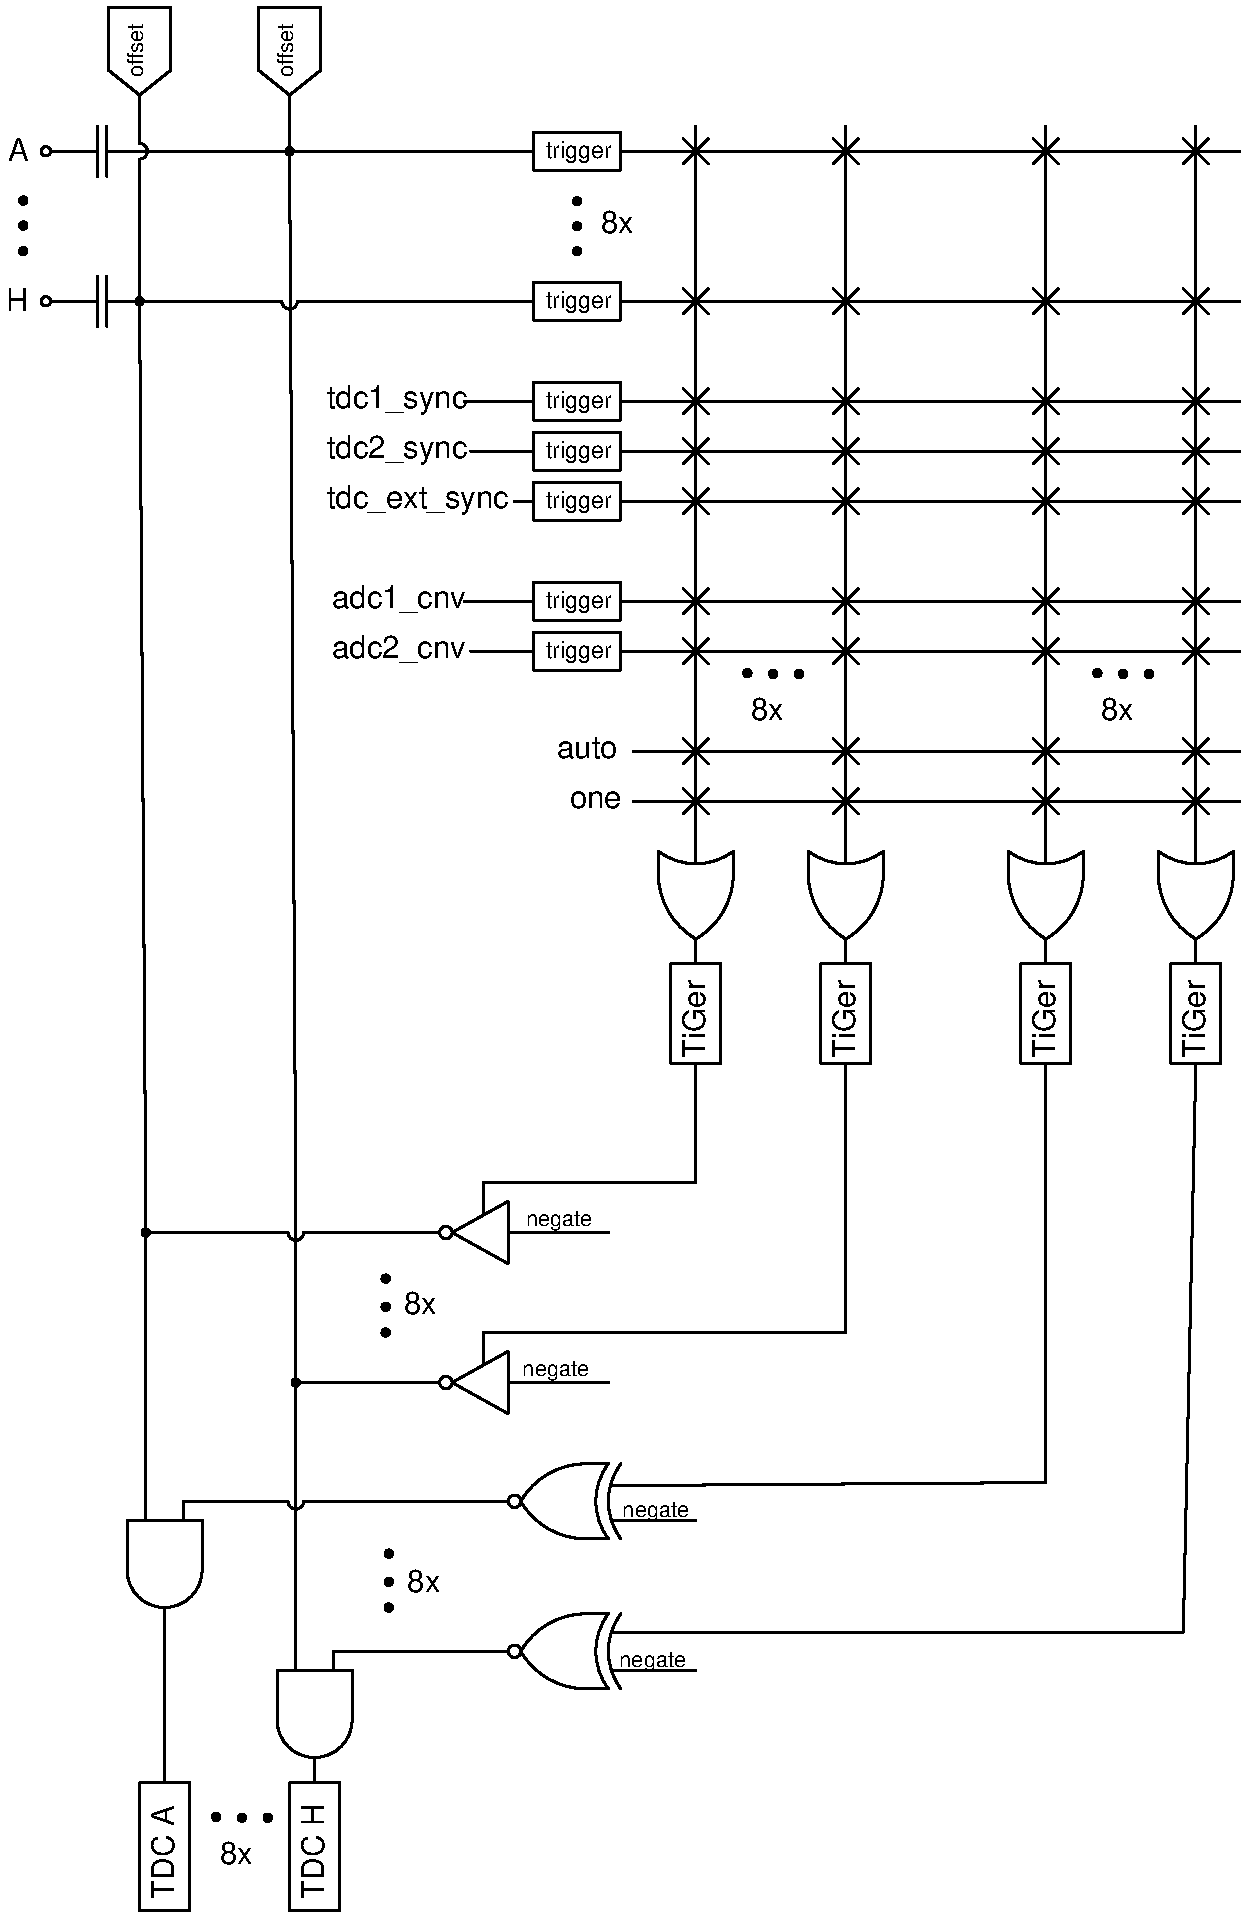
\includegraphics[width=0.7\textwidth]{figures/xhptdc8_trigger_matrix.pdf}
        }{
            \includegraphics[width=0.7\textwidth]{figures/xTDC4_tiger_matrix.pdf}
        }
        \caption{TiGer blocks can generate outputs that are also available on inputs.\label{fig:matrix}}
    \end{center}
\end{figure*}
%

Figure \ref{fig:matrix} shows how the TiGer blocks are connected. They can be triggered by an OR of an arbitrary combination of inputs, 
including the auto trigger. Each TiGer can drive its output to its corresponding LEMO connector. This turns the connector into a DC coupled output. 
Connected hardware must not drive any signals to connectors used as outputs, as doing so could damage both the \deviceName and the external hardware.
Pulses that are short enough for the input AC coupling are available as input signals to the \deviceName. 
This can be used to measure exact time differences between the generated output signals and input signals on other channels.

\ttinput{Tiger_Example.tex}	